\chapter{考察}
\label{考察}
\ref{validation}章では、修士作品の体験についてそれぞれの参加者がどのように体験していたかを紹介した。本章では、\ref{nerai}節で示した本作の体験における仮説と照らし合わせた上で、実際の作品体験について分析する。

\section{Familiar / Strange}
この作品におけるねらいは、トランジションの際の違和感が起点となって意識的な試行が引き出され、身体動作が変化することで一体感が生起することであった。また、バネ状に指の動きが連結されたシーン7では、はじめて指の動きが相互に干渉するようになり複雑度が増す。そのためそれを操る中で、より強い一体感(\textit{intimacy})を感じるのではないかと考えた。

\begin{figure}[H]
  \centering
  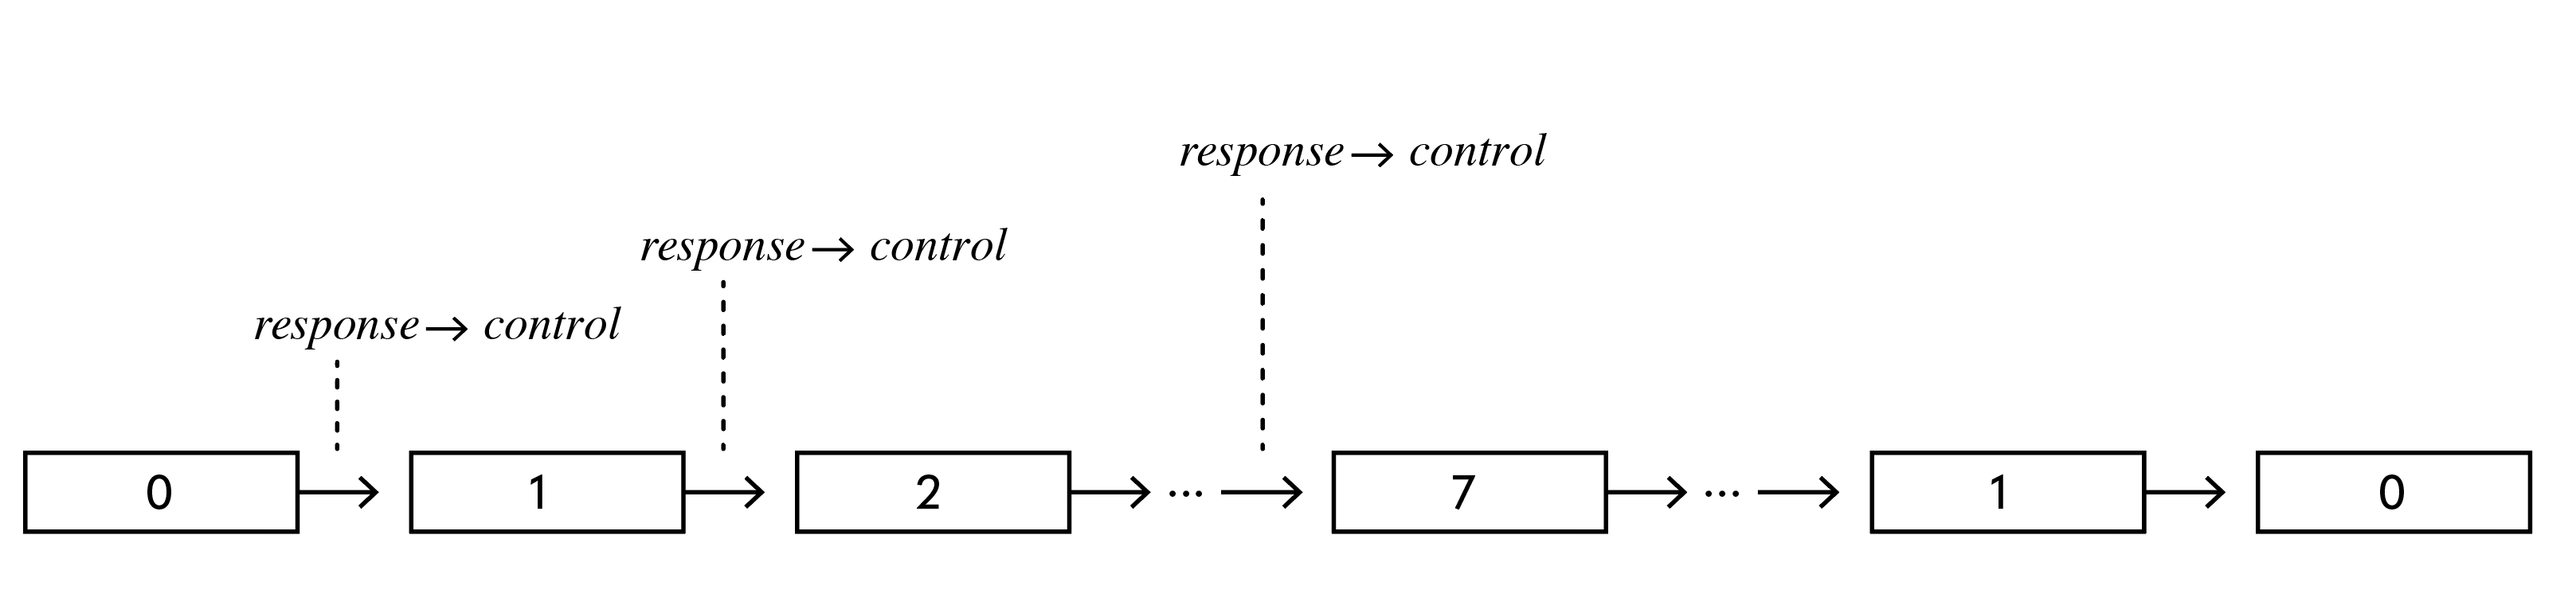
\includegraphics[width=15cm]{img/nerai_fs.png}
  \caption{《Familiar / Strange》のねらい(図\ref{fig:nerai_fs}を再掲)}
  \label{fig:nerai_fs_in_discussion}
\end{figure}

実際に、シーンの遷移に伴い\textit{response}の関係性が喚起される様子が確認された。
最初、グー、チョキ、パーの形を作ったり(参加者2)、手を握りしめたり、開いたり(参加者4)をしていたが、シーンが切り替わると、次第に指ごとに別々に動かすようになった。そのとき、「どれがどの場所なんだろう[...]っていうのを確認していた」(参加者1)、「指の位置がどういうふうに対応しているのかを確かめている」(参加者4)
というように、対応関係の確認を行なっていたことがわかる。これは、自分自身の動きではないトランジションによって、画面の中の手指と自分自身の対応関係が自明なものではなくなったことを示していると考える。

さらにシーン7では、バネ状の形を動かす上で最も動きを繊細に捉えることのできる縦方向に手指を動かすことを通して「気持ちよさ」を経験する、\textit{control}とみられる関係性が確認された。体験者2は、指の動きが先端と付け根の動きだけを追従した形に変化したシーン4から、さらにその動きが縦軸に拘束されたシーン5への変化を通して、ピアノを弾くときのように指を一本一本上下に動かすようになり、シーン7になってもその動きを続けている中で、手指を素早く動かしていても反応して動くことに「気持ちいい」と語っていた。また、参加者4はこの形状が画面の変化が最も大きいことから「気持ちいい動きをしてもらうことだけを考えてた」といって振り返っていた。

しかし、シーン7においては\textit{control}と思われる関係性が確認された一方で、そこに至るまでのシーンでは\textit{control}の関係にはほとんど至らなかった。参加者は、「どれがどの場所なんだろう」といった確認をしていたが、それ以上に何か目的意識を持って身体を動かしていたというようなコメントは少ない。しかし、目的意識を見出していた参加者は、変換された手指の形状に対して何かしらの「見立て」をしていた。参加者4はシーン4にて、指が縦方向の動きのみに拘束されてパタパタと上下する形になったとき「ピアノの演奏」のような身体感覚を想起していた。また参加者2は、シーン2や4をみて「植物か触角か、イソギンチャクみたいな感じ」に見立てると言ったように、「頭の中で既視感を作って」体験していたと振り返る。そうした見立てがなかなかできないシーンについては、「見たことない形のものだと[...]どうその曲線で遊ぶのかを見つけるのがなかなか大変」だったと語った。もし、見立てが可能な変換が行われていれば、この段階であっても\textit{control}の関係が生じていた可能性がある。

% 「見立て」は形に起因する見立ても存在するが、参加者4が身体の動きから「ピアノ」を連想していたように、過去に体験したことのあるような身体動作がこの場所で再演されることを通して、デジャヴのような感覚を引き起こす、「運動の見立て」の可能性も存在する。このように「見立て」が可能であることが、今後体験の中で目的意識や注意を自分で作って体験することにつながるのではないかと考える。

% また、最初の手指の形状からのトランジションによって親和性が失われていくことが確認された一方で、それ以降に親和性が失われていくような関係が芽生えてはいなかったのではないかと考えられる。参加者は作品の意図を知らされていないが、参加者2は、まさに「親和性」という言葉を用いて次のように体験を振り返っていた。
% \begin{quote}
%   ここら辺からちょっと違和感というか、親和性を確かめてたのに、その親和性から離れてく感じがしてた。今の自分の手と、こっち側の手の連動はしてるんだけど、離れている。自分の手じゃなくなる。
% \end{quote}
% そしてシーン7では「親和性」については諦めて、「身体的なところからは離れ」た存在となっていたことを振り返っていた。
% \begin{quote}
%   ここら辺からちょっと結構激しく手を動かし始めてた。[...]動きの精度を見てる。親和性はもう諦めて、動きの精度みたいなことを、よりシステムチックに見ちゃってる。身体的なところからは離れている、これはもう完全に。
% \end{quote}
% また、参加者4がシーン7において「気持ちいい動きをしてもらう」と語っていたことからも、自分の身体を動かしているというよりは、自分自身の身体ではないものを外から操っているような関係として認識していることが示唆される。そのため、体験の中で形状が変わった手指に対しても「まさに自分自身の身体である」と感じるような感覚が訪れ、それがトランジションによって崩壊する、といった違和感は現れない。実際、参加者4は度々「何も考えてなかった」瞬間があったことを振り返った。指がバネ状に積み重なっていくシーン6から7の遷移、そして手指の形にまた戻ってくるシーン1からシーン0への遷移の際である。このことから、すべてのトランジションが違和感を生み、ひいては意識的な試行を生むことに寄与するわけではないと考えられる。

加えて、作品のねらいとしたことがほとんど実現しなかった参加者もいた。
参加者3は最初、フレームを取るようなジェスチャーをしてトラッキングができていることを確かめていた。しかし手の形が変化し、異なる形状になっても「こうやってしたら(両手を開いて親指と人差し指をつなげ、三角形を作る)くっつくのかな」「(指を交差させて)こうやってやったら変わるのかな」と、「形を作る」ことに目的意識を抱いて体験していた。しかし、思うように形が作れないことから「反応がない」と感じられ、「飽きていた」とコメントしている。参加者3においてトランジションに伴う違和感が喚起されなかったのは、最初から「形を作る」ということに対して強い目的意識を抱いていたからではないかと考える。ジェスチャーを「入力」したはずなのに、何か意味を持った形が現れなかったことから「反応がない」と認識したのではないか。このことを踏まえると、この作品の体験においては、\textit{control}しようとすることだけに意識的になるだけではなく、グラフィックの変化に合わせて身体の動作を変化させていく必要があるのではないかと考えられる。

\section{Relation}
この作品におけるねらいは、ボールの操作やマトに当てるといった目的意識が起点となって意識的な試行が引き出され、その目的を達成するための技量を身につけることで一体感が生起することであった。またこの作品では、手そのもの、手とボール、ボールとマト、というように、段階的に緻密な運動の制御が求められることで、一体感(\textit{intimacy})が高まるのではないかと考えた。

\begin{figure}[H]
  \centering
  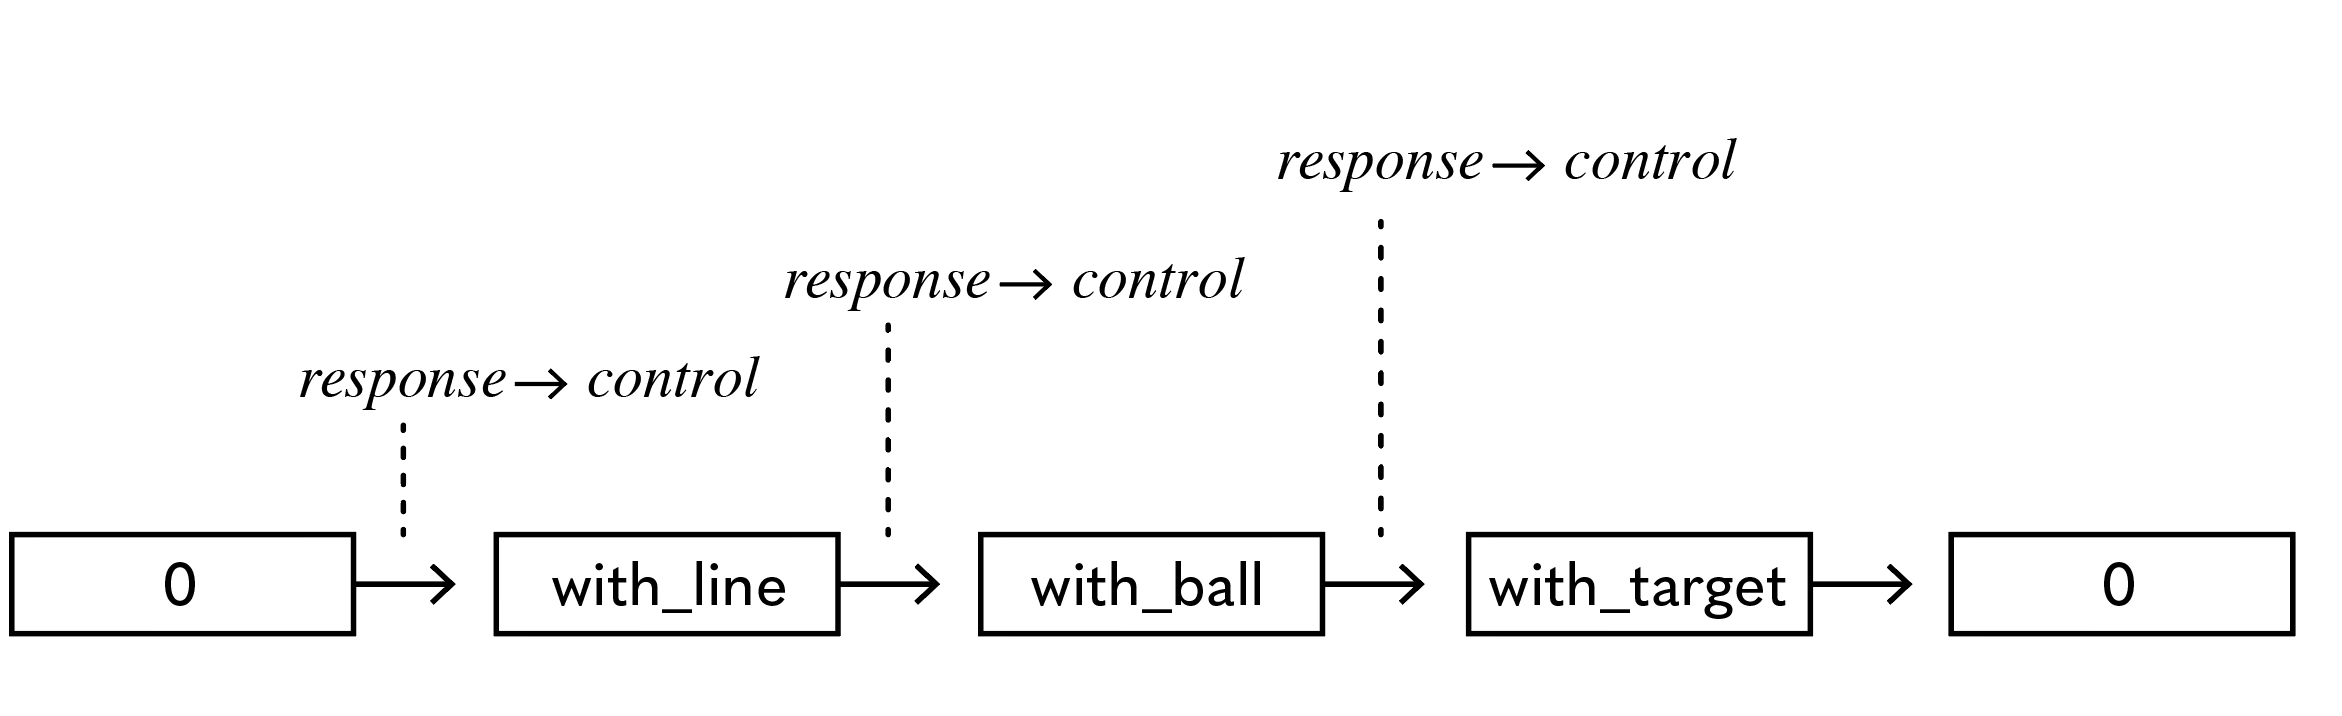
\includegraphics[width=15cm]{img/nerai_rl.png}
  \caption{《Relation》のねらい(図\ref{fig:nerai_rl}を再掲)}
  \label{fig:nerai_rl_in_discussion}
\end{figure}

結果、体験の途中で目的が変化することは確認されたが、「マトにボールを当てる」という目的に対して十分な技量を身につけた参加者は現れず、インタビューから一体感(\textit{intimacy})が生じたと取れるような発言は得られなかった。
《Relation》において最初、いずれの参加者もマトの存在や役割に気づかず、しばらくは「左にボールがあったら右の方に移動させようとか、右にあったら左に移動させてみよう」(参加者1)、「どれぐらいの動きでどれぐらいバウンドするのか」、「ボールをちょっと滞在させたい」「ちょっとなだらかな面を作ろう」(参加者2)、「(ボールを画面外に)落とさないようにしよう」(参加者3)、「ボールを投げ上げよう」(参加者4)といった目的を見出していた。そして、マトが出現してしばらくしてからボールがマトに偶然当たったり、狙って当てることを通して、マトの存在や役割に気づき、それ以降はいずれの参加者も「マトに当てる」ということを目的としていた。
しかしマトにボールが当たることはあっても、それは偶然であったり、随意であっても再現性が低く、「一体感」を感じられるほど器用に操れるようになった参加者はいなかった。
最後、全員が「マトに当てる」ということを目的としていたため、感想が「マトに当てられなかった」という経験が中心となったのではないかと考えた。

しかしこのことは、参加者が途中まで「一体感」感じられていたのに、目的が変化したことによって感じられなくなったためだと考えられる。例えば、参加者4は「目標」の変化が「気持ちよさ」の変化となっていたことについて語っていた。
\begin{quote}
  気持ちよさを感じるポイントは、ゲームを進めていく中で変化していった[...]最初は「球を上げる」っていう目標になって、それを達成する気持ちよさがあった。それを超えて、次の目標が見つかったときには、マトに当てないと気持ちよくない。(参加者4)
\end{quote}
このことから、それまで「気持ちよさ」を感じていた対象であっても、目的意識の変化によって「一体感」は失われることもあるのではないかと考えられる。
また参加者2は、《Relation》において「投げるときの反応が鈍」く、手指の動きの遅延やトラッキングの精度に対して「イライラ」、「もどかしい」と振り返っていた。これは、同じシステムを用いている《Familiar / Strange》においては述べられることがなかった内容である。ボールをタイミングよく動かす必要のある《Relation》においては、そうした誤差が前景化し、手指に対する「一体感が低い」と感じられたのではないか。

% 一方で、トラッキングが途切れることの多かった参加者4は、トラッキングが途切れてしまったこと自体に不快感を示さなかった。
% こうしたことを踏まえると、体験における「もどかしさ」とは目的意識との関係にあり、トラッキングの精度やトラッキングの可否の問題ではないと考えられる。また、作品がどのように動くのかについて、実際の正しい振る舞いについて理解することよりも、何かしらの納得感が現れることの方が重要であることが示唆された。

% 一方で、参加者3は、手指の対応関係については認識していたと振り返ったが、体験の途中でそうした対応関係とは関係なく、手のひらを上に向けて掬い上げるような動きをしていた。慎重に画面の中で行われていることを観察した上で身体を動かすというよりは、自分の表現したいことを身振りでジェスチャーするような体験であったと言える。本作品は、手指の身体動作が全て認識されて動作するため、あらゆる動作を受け付けるという点で、探索をする上で適度に抽象的であると考える。ただしその一方で、慎重になることについては必ずしも必ずしも喚起出来ているわけではないということがわかった。しかし、その設計は慎重に行う必要がある。なぜなら注意を喚起する構造を設計することは、抽象度を高めることとトレードオフの関係となってしまうことがあるためである。

\section{Felsのモデルの拡張}
ここまで、Felsのembodimentの分類や\textit{intimacy}の生起という観点から、本作品が目指す「人馬一体感」を捉えようとしてきた。しかし、この作品において重要な体験でありながら、Felsの定義したカテゴリを用いるだけでは捉えきれなかったことがある。それは、手指の構造が変化することをきっかけに生じる、「身体動作の変化」である。本作品においては、体験中常に身体動作とグラフィックの連動性は担保されている。しかしながら、一度構造が変化すると自分の動きとの対応関係が曖昧になり、「動いてはいるが、自分が動かしている」という感覚が薄れていく。そして、改めて「どこがどのように対応しているのか」ということを動きの中で確認することを通して構造を把握し、再び「自分が動かしている」という感覚が芽生える。このとき、Felsのカテゴリで言えば「自分の動きによってそれが動いている」という点において\textit{control}の関係性であるということができるが、一方で「自分が動かしている」という感覚を得るためには確認の動作が必要であり、どのようにそれが振る舞うのかを理解して、それに合わせた身体の動かし方をする、すなわち対象に帰属(\textit{belonging})する必要がある。

この作品において生じている一体感とは、単に自分の思い通りに制御しようとするだけで生起するものではなく、作品の振る舞いを意識的に観察しながら、それに合わせて動作を変更しない限り起こらない。つまり、\textit{control}すると同時に\textit{belonging}することをなしには一体感が生起しない。実際、参加者3は「ジェスチャー」のような動きをしようとしたことに対して、作品からの影響を受けなかったことから一体感が生起しなかった。こうしたFelsの定義に収まりきらないところに、「人馬一体感」があるのではないか。


% 《Strange / Familiar》で見られた「どのように振る舞うのかを確かめる」、《Relation》に見られた「当てようとしても、思うように当たらない」といったときの関係性は、
% この作品における一体感を捉える上で重要であるが、それはFelsのいう\textit{control}にも、\textit{belonging}にも該当しない。

% このときの対象との関係性を、仮に「\textit{grasp}」とした。

% \section{新たに重要だと思われた指標}
% \subsection{見立て}
% 目的意識を抱いていた参加者は、何かしらの「見立て」をしていたことがわかった。参加者4は、指が縦方向の動きのみに拘束されてパタパタと上下する形になったときに、ピアノの演奏のような身体感覚を想起していた。また参加者2は、「頭の中で既視感を作って」体験していたと振り返る。こうした「見立て」が生じることは、体験する人がそこに目的意識を見出して、対象を捉えようとすることの表れと考えられる。

% 「見立て」は形に起因する見立ても存在するが、参加者4が身体の動きから「ピアノ」を連想していたように、過去に体験したことのあるような身体動作がこの場所で再演されることを通して、デジャヴのような感覚を引き起こす、「運動の見立て」の可能性も存在する。このように「見立て」が可能であることが、今後体験の中で目的意識や注意を自分で作って体験することにつながるのではないかと考える。

% \subsection{連動性の担保}
% 「思い通りに動く」とは「連動性が担保されていること」ではないか、という仮説が新たに生じた。「思い通り」という言葉は、相手に命令する立場からすると、期待している結果と実際の挙動が一致している際に生じるが、「control」の状態下での「思い通り」とは、参加者2が体験を振り返るコメントにもあるように、「トラッキングができて」いて、「時差を極力なくし」た動きが「自分の思い通りの動きになってくれる状態」、すなわち「連動性」ではないかということが示唆された。その上で、「Belonging:帰属感」のようなintimacyが生じるためには、その動きがさらに細かく制御できていることが重要ではないかと考えられる。

% \section{総括}
% 2つの作品では、それぞれ異なる性質の\textit{grasp}を喚起することが出来ていたことが明らかとなった。しかしその一方で、\textit{belonging}や\textit{control}といった関係性が芽生えていたと判断できるような状況が少なく、\textit{grasp}こそが親密さを高める要素として寄与していたのかについては、検証することが難しいと考えた。

% そこで、今後作品の体験を発展させる上で、\textit{control}や\textit{belonging}を発生させる可能性がある表現を、今回の分析を踏まえて列挙する。

% \begin{quote}
%   \begin{enumerate}
%     \item 「見立て」が可能な作品は、さらに目的意識を設定しやすく\textit{control}の関係性が芽生えることが考えられる。そのためには積極的に「見立て」が生じる状況を設計するというアプローチもありうるが、プロトタイピングでもあったように作品体験の複雑度を上げるような展開のさせ方も考えられる。今回の「Familiar / Strange」では、トランジションの過程でこの「見立て」が特に起こり得ず、目的意識を抱きづらい状況が続いていたことが課題として挙げられる。
%     \item 「マト」の存在は、全体的に強い目的意識を喚起させる表現となっていた一方で、体験者が目的意識を設定する余地をなくしてしまっていたことが考えられる。これは、「ゲーム性」を追及するのではない方法で目的意識をいかに設計していくのかという、遊びに関する議論とも接続する。前の要素とも関連するが、例えばオンスクリーン表現ではなく、フィジカルな表現で関係性の複雑度を上げるなど、注意を向ける対象の増やし方には検討の余地があると考える。
%     \item 体験の中で、抱いていた関心に対して試行しきることがないままに体験が終了していたことがあった。トランジションは作品の構造を示し、段階的に注意を向けることに寄与していた一方で、徐々に展開されてしまうことが集中を途切れさせる原因にもなっていたのではないかということが課題として挙げられる。
%   \end{enumerate}
% \end{quote}

\section{\textit{grasp}について}
そのため、「人馬一体感」を捉えるためには、「操作はしているが、自分が動かしているという感覚がない」という人と対象との関係を捉えるカテゴリが必要となると考えられる。そこで、本研究ではそのカテゴリを\textit{grasp}と名付けた。
graspは「把握」を意味する動詞であり、\textit{control}に向けて、対象の「思い通りにいかなさ」から影響を受けながら、折り合いをつけるために試行錯誤をしている状態である。本作品においてこの\textit{grasp}という関係性は、形が変化してから、身体動作を変化させていくまでのあいだに見られる。参加者1が《Relation》について、「ちょうどいい難易度で、所々面白かったな。[...]その面白かったなっていうのは、なかなかうまくいかんなっていう面白さ。[...]わかっちゃいるけど、うまくいかんなっていうような。」と語っているように、仕組みについては理解した上で、それでも自分の思うようにいかないような経験をしているとき、この\textit{grasp}が生じているのではないかと考えられる。

実際の体験の様子を分析した結果と、ここで新たに導入した\textit{grasp}を用いて体験を再び説明すると、作品での体験はそれぞれ次のように説明できる。

\begin{figure}[H]
  \centering
  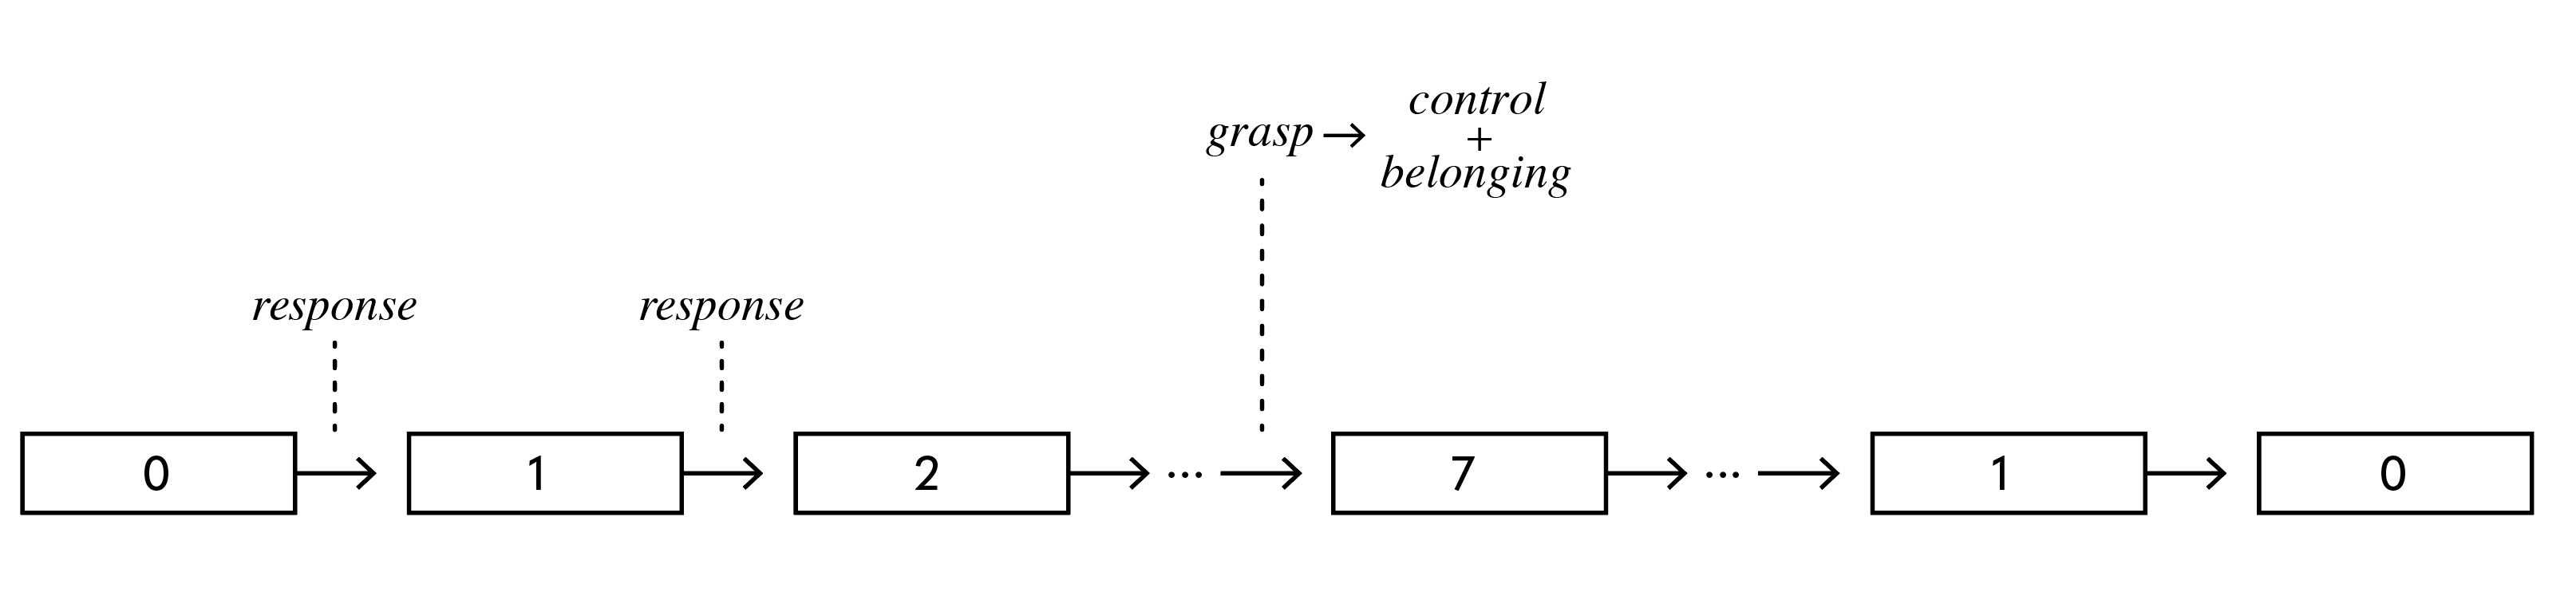
\includegraphics[width=15cm]{img/result_fs.png}
  \caption{\textit{grasp}を用いた《Familiar / Strange》の体験の説明}
  \label{fig:result_fs}
\end{figure}

《Familiar / Strange》においては、手指の変換だけでは「どこがどの指なのか」と確認することはあっても、それを踏まえて何か目的意識を抱くことは難しい。だが、シーン7のように複雑度が増し、動かすときに緻密な制御が求められるようになると、\textit{control}と取れるような経験があった。そして、この体験に至るためにはそれまでの\textit{response}を通して動きの仕組みについては理解していて、そうした経験を組み合わせることで、段階的にシーン7でその構造に合わせた動きができるよう、身体の動作が変化する\textit{grasp}の関係が間にあったと言える。また、そうした過程を経て一体感が生じるまでには、自分自身が身体の動かし方を変化させることが起きている。このことから、シーン7での一体感においては、\textit{control}に加えて\textit{belonging}も生じていると考えられる。

\begin{figure}[H]
  \centering
  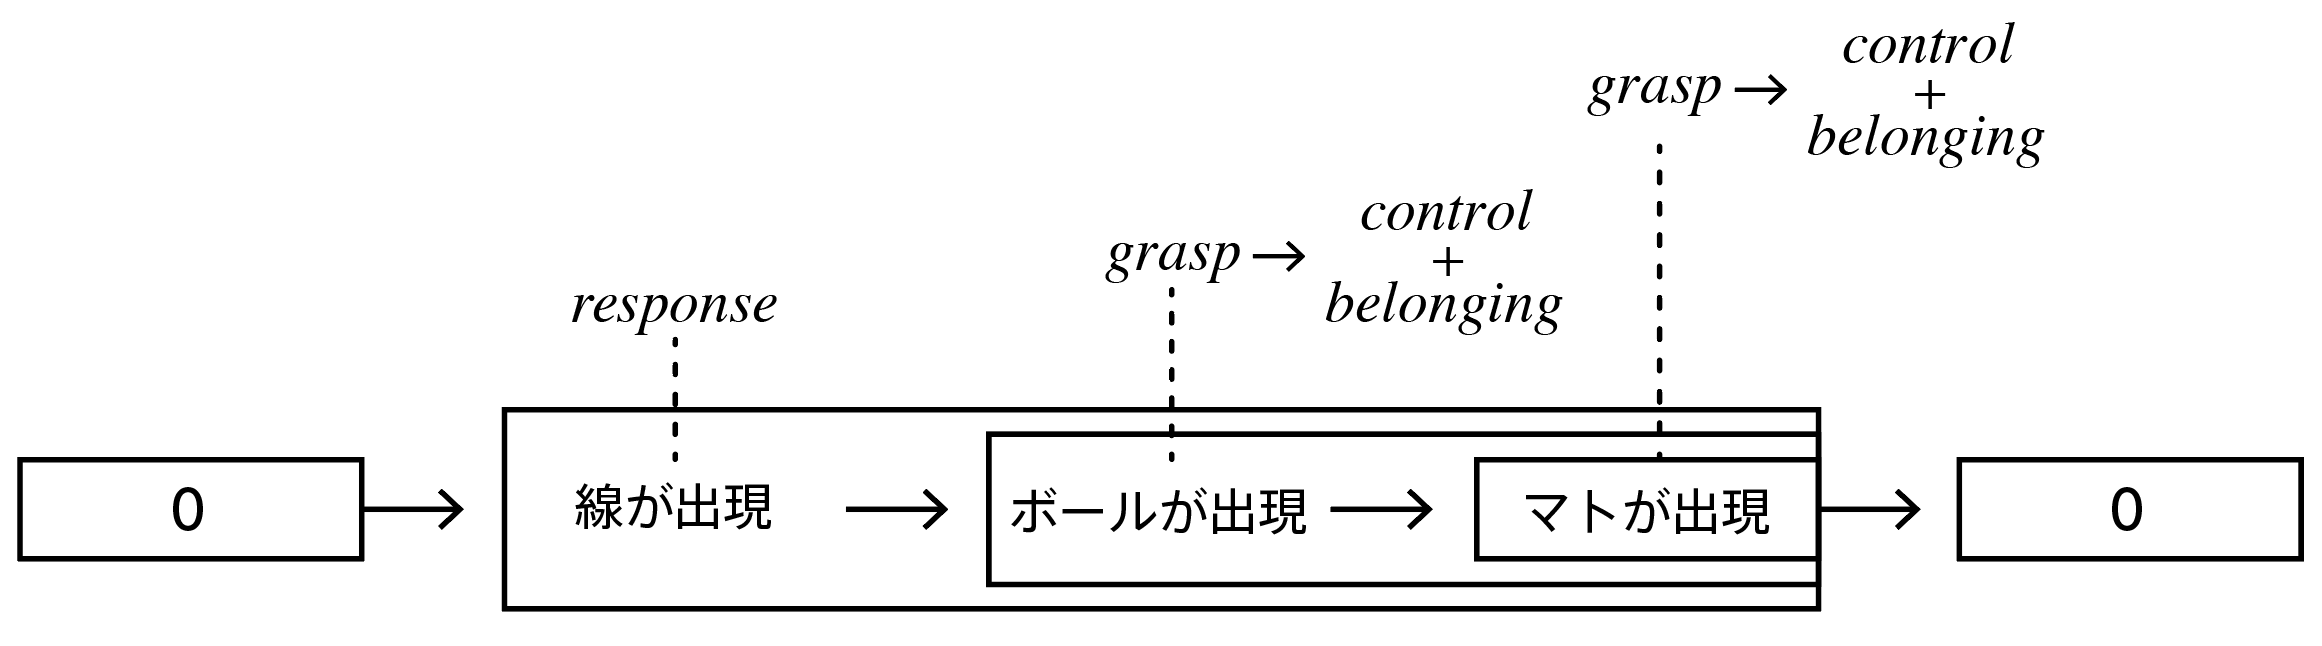
\includegraphics[width=15cm]{img/result_rl.png}
  \caption{\textit{grasp}を用いた《Relation》の体験の説明}
  \label{fig:result_rl}
\end{figure}

《Relation》においても、手指が変換していくだけでは目的意識を抱きづらく、\textit{response}はあっても\textit{control}の関係性には至ることが難しいのではないかと考えた。しかしボールが現れると、それを飛ばす、左右に転がすといった目的意識を抱く。そしてそれは、器用に扱えるようになるには習熟が必要である。そのため、ここに\textit{grasp}が生じ、その結果として\textit{control}と\textit{belonging}が同時に生起するといった状態が生じると考えられる。

% \textit{grasp}とは例えば、ギターの習得過程において、弾きこなしたいフレーズを定め、それを達成するまでに試行錯誤をし、達成できるようになるまでの期間である。熟達した状態では、熟達する前とは違う視座でものごとを捉えられるようになり、また違う対象に注意が向くようになると、ギターと人との間に別の\textit{grasp}が芽生える。
% またあるいは、\textit{grasp}の過程で、対象と向き合い続ける過程の中でその解像度が高まり、当初目指していたこととは違うことに興味を抱く(セレンディピティ)ことでも、別の\textit{grasp}が芽生える。

% ここまで具体例を通してみてきたように、\textit{grasp}は、ギターと人との関係において一度だけ生じるのではなく、注目する対象が定まれば何度でも生じる。

% \textit{grasp}について、本研究では次のように定義する。

% \begin{quote}
%   \textbf{人と対象との関係の中で、人が対象の中に注意や目的意識を抱きながら、意識的に試行する期間}
% \end{quote}

% graspは「把握」を意味する動詞でもあるが、ここで「動作」ではなく「期間」とした。その理由は、「意識的に試行する」とき、同時にその結果を受けて気づきを得たり、その気づきをもとに新たな関心を抱くといった、単に自分が行為しているだけではなく、対象から影響を受けながら次の行為が決まってくるようなフィードバックループの構造があると考えるためである。「grasp=把握」という言葉についても、単に「ものを掴む」という意味だけでなく、「理解」の意味があることは、対象について一方向に働きかけているのではない様子が現れているのではないだろうか。

